\chapter{Paper 2}\label{sc:p2}
\textbf{\Large Switched Capacitor Analog Modulo Integrator For Application
  In Open Loop Sigma-Delta Modulators}\\
\indent Carsten Wulff, {\O}ystein Knauserud, Trond Ytterdal\\
\indent Analog Integrated Circuits and Signal Processing\\
\indent Springer Netherlands\\
\indent ISSN 0925-1030\\
\indent Volume 54, Number 2, Pages 121-131 Febuary 2008\\
\indent DOI 10.1007/s10470-007-9084-2\\

\renewcommand\myfigname{p4fig:}
\renewcommand\myeqname{p4eq:}

\section*{Errata}
\begin{itemize}
\item Section 5.3.3, 5`th line: an $\rightarrow$ a
\item Section 5.3.3, second to last paragraph: We say that
  quantization noise can have codes that span the range of the
  quantizer, but this is incorrect. Quantization noise is limited to
  1LSB, so the maximum difference between two output codes with the same analog
  input is
  1LSB. This assumes that thermal noise is less than 1LSB. Thus, the
  statment in the second to last paragraph is not valid for quantizers with more than
  on bit.
\end{itemize}

%\section{Abstract}
\begin{abstract}
%------------------------------------------------------------------------
We introduce the switched capacitor analog modulo integrator, which to
our knowledge is a new circuit. We introduce
the amplitude modulated open loop \SD modulator (OLSDM), which is an analog modulo integrator
followed by a quantizer and a modulo differentiator. The mathematical
equivalence between low pass \SD modulators and OLSDM is
explained. Behavioral simulations confirm the equivalence. The
necessary circuit, a switched capacitor analog modulo integrator, is explained in detail. 
Behavioral level simulations in SPICE of the analog modulo
integrator verify the function, and prove the concept of
amplitude modulated OLSDM.

\end{abstract}

%\keywords{
\paragraph{Keywords}
 \SD Modulators, Switched Capacitor Circuits, Analog Modulo Integrator

%}
%\end{opening}        

%-------------------------------------------------------
\section{Introduction}
%-------------------------------------------------------
\SD modulators have become a natural choice for
analog-to-digital conversion in applications with low to medium
bandwidth 
and high resolution.  
The \SD modulator shapes the spectral density of the quantization error of
 data converters. 
The quantization error, or as it is often called, quantization noise,
is the error introduced by converting a continuous value signal into a
discrete value signal. This error is often considered to have uniform
spectral density, or in other words, be a white noise source. The
conditions for considering quantization error as a white noise source
was covered in \cite{widrow56}.   


The conventional low-pass \SD modulator (L-SDM) in its simplest form consists of an
integrator followed by a quantizer. The quantized signal is fed back
to the input through a digital-to-analog converter (DAC) and subtracted from
the input. The transfer function of the modulator is different for the
input signal and the quantization noise.  \footnote{This assumes a linear model of the quantizer,
  since the transfer function is only defined for a linear system} The input
signal will undergo an integration followed by a
differentiation and have a transfer function of one. The quantization noise will be
differentiated and thus high pass
filtered.

In an ideal world, with no voltage swing limitations, an L-SDM system
could be implemented by an integrator 
followed by a quantizer and a differentiator, but since supply voltage
is limited in electronic circuits, and an integrator  
has infinite dc gain, it is difficult to implement. Somehow
the output swing of the integrator has to be limited. Feedback is
normally used to limit the output swing of the integrator. 
 
There are many different types of \SD modulators. In this
paper we discuss a small sub group that we denote Open Loop \SD
Modulators (OLSDM). We define an OLSDM as: Any \SD modulator that does
not have feedback of the quantized modulator output signal.

One of the first suggestion of an OLSDM can
be found in \cite{claasen80}. Although there is no system
implementation they explain a method that avoids the feedback
DAC. More recently there have been others like the Frequency
\SD Modulator (FSDM)  in \cite{hovin97} and
\cite{wismar06}.

In the FSDM a voltage to frequency converter, a voltage controlled
oscillator (VCO), was used in place of the
integrator, and it was shown in \cite{hovin97} that the pre-processing
in FSDM is equivalent to modulo integration. The FSDM could be identified
as a frequency modulated OLSDM. 


In \cite{wisland02} they introduced the
non-feedback \SD digital-to-analog modulator where the
integrator was implemented as a digital modulo integrator. 

 In the
 past the noise shaping of \SD modulators has been combined with the
 high speed of pipelined ADCs. In \cite{brooks97} a second
 order five bit \SD Modulator was cascaded with a 12 bit
 pipelined ADC. The output of the \SD Modulator was combined with the
 output of the pipelined ADC to generate the digital output word. We
 wanted to investigate 
 whether one could avoid any interaction, with the exception of the
 input and output signals, between the \SD Modulator and the pipelined
 ADC in such a
 system. The question was; could one pre-process the input signal to
 implement the
 sigma, quantize and do post-processing to perform the delta,
 without interaction between the 
 sigma and the delta. The block diagram of such a system is shown in Figure \ref{p4fig:olsdm}

\begin{figure}[htbp]
\centerline{ 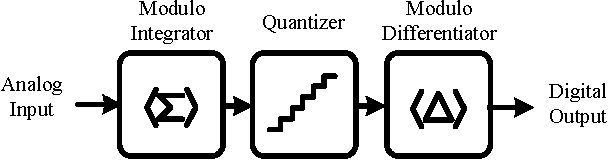
\includegraphics[width=\myfigwidth]{graphics/olsdm-sc}}
  \caption{First order OLSDM block diagram}
  \label{p4fig:olsdm}
\end{figure}


We knew from \cite{wisland02} that the open loop
 \SD modulator was  possible when all blocks were digital, by using modulo
 integration, quantization and modulo differentiation. However, in an
 analog-to-digital OLSDM the modulo integration would have to occur in
 the analog domain. 
We were unable to find any
published circuit that matched our requirements for an analog modulo integrator. Accordingly, the switched
capacitor analog modulo integrator was developed, which we present
here. To our knowledge, this switched capacitor analog modulo
 integrator is a new circuit.


In Section \ref{p4modolsd} we elaborate on the mathematical
equivalence between OLSDM and L-SDM,  which is supported by behavioral
simulations in Matlab in Section \ref{p4matlab}. Quantizer non-linearity
and common errors are also discussed in Section \ref{p4matlab}. In Section \ref{p4modint}
we introduce the analog switched capacitor modulo
integrator. Behavioral level simulations with a SPICE macro model of
the analog modulo integrator and the OLSDM are presented in Section
\ref{p4simulation}. 

%-------------------------------------------------------
\section{Open Loop \SD Modulator} \label{p4modolsd}
%-------------------------------------------------------

The most basic low pass OLSDM is an integrator, followed by a
quantizer and a differentiator as illustrated by Figure \ref{p4fig:olsdm}. The
input signal is integrated and afterwards differentiated, hence the
output is equal to the input, assuming a linear system. The quantization error added by the
quantizer is differentiated thus high pass filtered. To limit the
swing in the analog domain we use a modulo operation at the output of
the integrator. The inverse operation, which is also a modulo
operation, is performed in the digital domain after the
differentiator. A modulo operation is trivial to implement in the
digital domain. The analog modulo
operation is not trivial, and it has previously been implemented as a
voltage to frequency converter in \cite{hovin97} and \cite{wismar06}. 


The equivalence of L-SDM and OLSDM was shown in \cite{wisland02}. Here
we
endeavor to explain the equivalence more intuitively.  

The OLSDM has been modeled as a piecewise linear system.
The modulo
operation is a non-linear operation, but it can be seen as a piecewise
linear system if we ignore the discontinuities when the modulo
operation occurs. 
The quantizer has been modeled as a linear addition of noise. Figure
\ref{p4fig:modolsd} shows the complete modulator. 

\begin{figure}[htbp]
\centerline{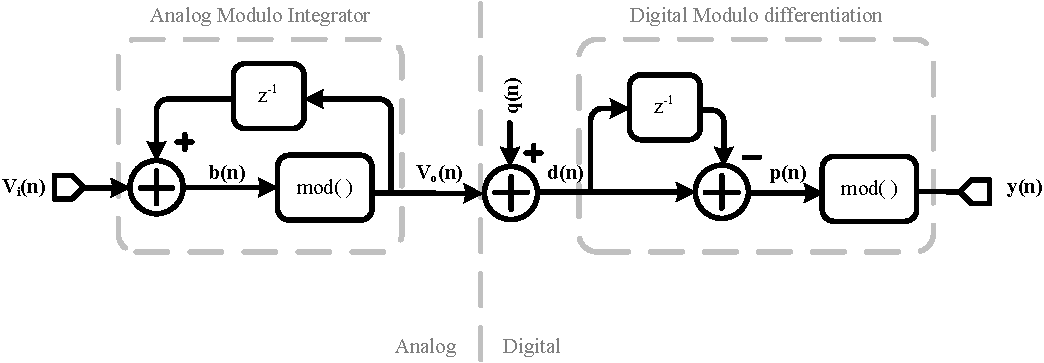
\includegraphics[width=\myfigwidth]{graphics/modolsd}}
  \caption{Piecewise linear model of the OLSDM}
  \label{p4fig:modolsd}
\end{figure}


The input signal to the modulator is $V_i(n)$, where $n$ is the sample
index. A signal with sample index $n$ is the current sample while
$n-1$ is the previous sample. The input is added to the previous
output of the integrator, $V_o(n-1)$, resulting in $b(n)$. The signal
$b(n)$ is subjected to modulo operation with $V_o(n)$ as a result.
$d(n)$ is the sum of $V_o(n)$ and the quantization noise, $q(n)$. The
differentiator output $p(n)$ is $d(n)$ minus the previous quantizer
output $d(n-1)$. To get the output, $y(n)$, $p(n)$ is subjected to a
modulo operation.  In this system the second modulo operation cancels
the first modulo operation and we have a system that is equivalent to
an L-SDM.  The equations in more detail follow.  

We define the previous output from the integrator as
\eqn{
V_o(n-1) \in \langle -V_{ref}, V_{ref} \rangle
}
and the input signal as
\eqn{
\label{p4eq:rangeinput}
V_i(n) \in \langle -V_{ref}, V_{ref} \rangle
}
where $V_{ref}$ is the reference voltage.

We know that after integration, but before the modulo operation, we get
\eqn{
\label{p4eq:modintb}
b(n) = V_i(n) + V_o(n-1)
}
where $b(n)$ will be bounded by
\eqn{
b(n) \in \langle -V_{r}, V_{r} \rangle
}
where $V_r = 2V_{ref}$.
The modulo operation is used to reduce the output swing to $V_o(n) \in \langle
-V_{ref}, V_{ref} \rangle$. The modulo operation subtracts or adds
 $V_r$, depending on the value of the
summation in \req{modintb}.
The next output from the integrator can be
written as 
\begin{numcases}{V_o(n) = }
\label{p4eq:modint}
b(n) + V_r & $b(n) \in \langle -V_r, -V_{ref}]$\nonumber\\ 
b(n)  & $b(n) \in \langle -V_{ref} , V_{ref} \rangle$ \nonumber\\
b(n) - V_r & $b(n) \in [ V_{ref}, V_r \rangle$
\end{numcases}
Accordingly \req{modint} is the equation for a modulo integrator.
After quantization the input to differentiation will be
\eqna{
d(n) &{}={}& V_o(n)+ q(n)\nonumber\\
d(n-1) &{}={}& V_o(n-1) + q(n-1)
}
where $q(n), q(n-1)$ are the quantization errors. 
The the output of the differentiator is
\eqn{
\label{p4eq:p(n)}
p(n) = d(n) - d(n-1)
}
If we in \req{p(n)} insert for $d(n)$, $d(n-1)$, $V_o(n)$ and set $e(n) = q(n)-q(n-1)$ the expression becomes
\begin{numcases}{p(n) = }
\label{p4eq:z2}
V_i(n) + V_r + e(n) &$V_i(n) \in \langle -V_{ref} , 0 \rangle$\nonumber\\
V_i(n) + e(n) &$V_i(n) \in \langle -V_{ref} , V_{ref} \rangle$\nonumber\\
V_i(n) - V_r + e(n) &$V_i(n) \in \langle 0 , V_{ref}  \rangle$
\end{numcases}

The bounds of $V_i(n)$ in \req{z2} are derived from the possible input
signal values for the modulator to reach the states in
\req{z2}. Consider the first case where 
\eqn{
p(n) = V_i(n) + V_r + e(n), V_i(n) \in \langle -V_{ref} , 0 \rangle
} Here $V_r$ has been added,
thus 
\eqn{
b(n) \in \langle -V_r, -V_{ref}]
} from \req{modint}. For b(n) to
have these bounds 
\eqn{
V_i(n) \in \langle -V_{ref}, 0 \rangle}
 and
\eqn{V_o(n-1) \in \langle -V_{ref}, 0 \rangle}
This is sufficient to
ensure the bounds of $p(n)$ in case 1 in \req{z2}  are \[p(n) \in [
V_{ref}, V_r \rangle\] Thus when we apply another modulo operation we
get 
\begin{numcases}{y(n) = }
\label{p4eq:yn}
V_i(n) + V_r - V_r +e(n)   &$V_i(n) \in \langle -V_{ref} , 0 \rangle$\nonumber\\
V_i(n) + e(n) &$V_i(n) \in \langle -V_{ref} , V_{ref} \rangle$\nonumber\\
V_i(n) -V_r +V_r + e(n) &$V_i(n) \in \langle 0 , V_{ref}  \rangle$
\end{numcases}
and for all cases in \req{yn}, $y(n) \in \langle -V_{ref} , V_{ref}
\rangle $. Equation \req{yn} can be expanded into \[y(n) = V_i(n) + q(n) - q(n-1)\]
Which result in the well known equations
\eqn{
\frac{y(z)}{V_i(z)} = 1 \:,\:
\frac{y(z)}{q(z)} = 1- z^{-1}
}
The transfer function from the input signal to the output is one, which
is the same as for an L-SDM, although often the transfer function of an L-SDM from input to
  output contains a time delay, $y(z)/V_i(z) = z^{-1}$. The quantization error is
differentiated, thus first order high pass filtered. This proof can be
extended to higher order modulators. 

%-------------------------------------------------------
\section{Behavioral Simulations In Matlab} \label{p4matlab}
%-------------------------------------------------------
The behavioral simulations presented here are an
implementation of the equations explained in the previous
section. \footnote{The Matlab code for the first and second order
  OLSDM can be downloaded from http://www.nextgenlab.net/olsdm}

%-------------------------------------------------------
\subsection{First And Second Order OLSDM}
%-------------------------------------------------------
 A first and second order
OLSDM and an oversampled quantizer without noise
shaping were modeled and simulated in Matlab. The oversampled quantizer without noise shaping was included
to compare ideal results with the simulated results. All quantizers
were implemented as 7 bit quantizers.  An oversampling ratio
(OSR) of 8 was chosen. An overview of the system can be seen in Figure
\ref{p4fig:matsys}. 

\begin{figure}[htbp]
\centerline{ 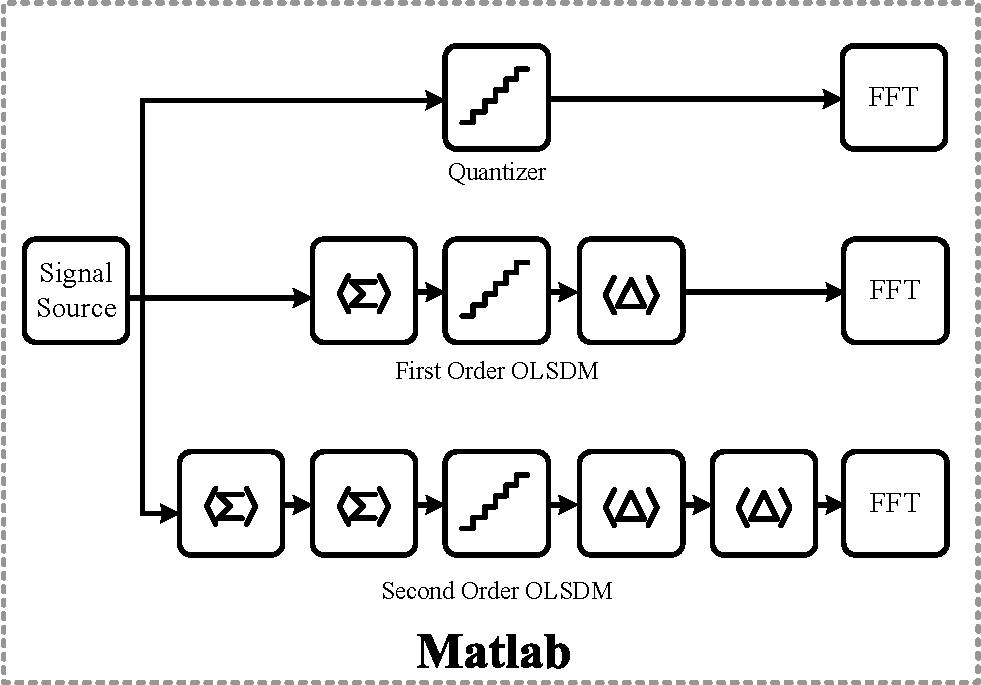
\includegraphics[width=\myfigwidth]{graphics/matsys}}
  \caption{Overview of behavioral level simulation system}
  \label{p4fig:matsys}
\end{figure}


The ideal signal to noise and distortion ratio (SNDR) for the
different cases are shown in Table \ref{p4tab:idealsndr}. The ideal SNDR
are based on equations from \cite{johns}.

\begin{table}[htbp]
\caption{ Ideal SNDR for 7 bit quantizer, OSR=8  }
\begin{tabular}{ccc}
\label{p4tab:idealsndr}
 Noise Shaping & Improvement (dB)  & Total (dB) \\ 
\hline None & $10 \times \log(OSR)$ &  52.9 \\ 
First order & $30 \times \log(OSR) - 5.17$ & 65.8 \\ 
Second order & $50 \times \log(OSR) - 12.9$ & 76.1 \\ 
\end{tabular} 
\end{table}

The equations for the OLSDM were implemented as specified in the previous section
with one exception. We chose to implement the quantizer using unsigned
integer outputs, the output ranging from 0-127. With this implementation $d(n)$ has a dc
offset. The differentiator is a high pass filter and
removes this dc offset.  For the modulo operation to work,
a dc offset was added after the differentiator to restore the correct
common mode. In the second order OLSDM a dc offset was added after
both differentiators. 

The sampling frequency was chosen arbitrarily at 1MHz and the input
signal was chosen according to the rules of coherent sampling
\cite{IEEE-1241}. In Matlab the sampling frequency is of no 
importance, we could just as well have used normalized
frequencies. However, these simulations will be compared to SPICE
simulations, and in SPICE the sampling frequency is of importance. The
input frequency was $f_{in} = 6164.6Hz$ and 
$2^{15}$ samples of the output, $y(n)$,  were calculated.

The input signal to the OLSDM must be limited, as specified in equation
\req{rangeinput}. It turns out that \req{rangeinput} is incorrect when
we deal with a finite resolution quantizer, which we will discuss in
the next section.
For the remainder of this paper the input signal amplitude has been
fixed at 0.9FSR, unless otherwise specified.
As a consequence SNDR will be 0.91dB lower than ideal cases in Table
\ref{p4tab:idealsndr}.  

The outcome of simulations are summarized in Table
\ref{p4tab:olsdmsndr}. Both the second order OLSDM and the first order
OLSDM have approximately the same SNDR as the ideal modulators. When we
remove the effects of reduced input amplitude we are left with an
error of  $+0.2dB$ for no noise shaping,  $+0.01dB$ for first order
OLSDM, and $-0.19dB$ for second order OLSDM, which is within the
errors of the SNDR extraction.  

The Fast Fourier Transform was used to
extract the SNDR, the FFTs can be seen in Figure \ref{p4fig:olsdmat} and
Figure \ref{p4fig:olsdmat2}. The light gray spectrum in the figures are the
FFTs of the ideal 7 bit quantizer, which is the same for the two figures. 

\begin{table}[htbp]
\caption{SNDR of OLSDM modulators with $2^{15}$ point FFT}
\begin{tabular}{cccc}
\label{p4tab:olsdmsndr}
 Noise Shaping & Total (dB) & Difference from Ideal (dB)\\ 
\hline
None & 52.2 & -0.7 \\ 
First order &  64.9 & -0.9 \\ 
Second order & 74.9 & -1.1 \\ 
\end{tabular} 
\end{table}

\begin{figure}[htbp]
\centerline{ 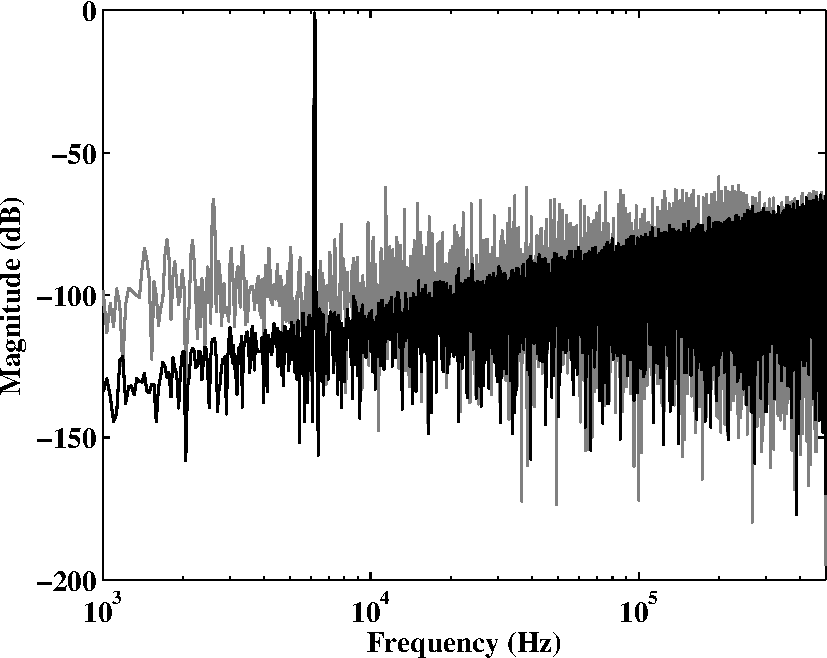
\includegraphics[width=\myfigwidth]{graphics/olsdmat} }
\caption{$2^{15}$ point FFT of the first order OLSDM output}
 \label{p4fig:olsdmat}
\end{figure}


\begin{figure}[htbp]
\centerline{ 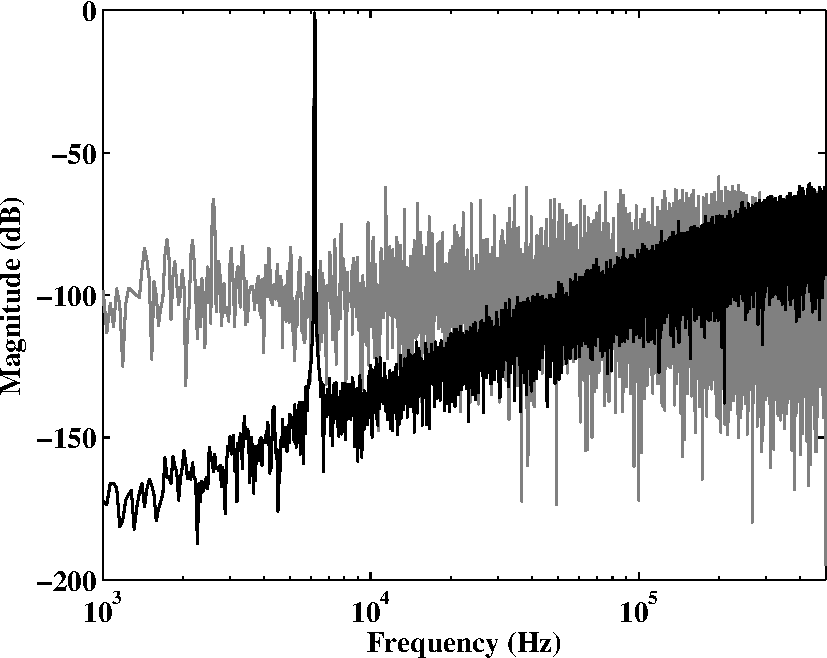
\includegraphics[width=\myfigwidth]{graphics/olsdmat2} }
\caption{$2^{15}$ point FFT of the second order OLSDM output}
 \label{p4fig:olsdmat2}
\end{figure}

%-------------------------------------------------------
\subsection{Input Signal Amplitude Limitations}
%-------------------------------------------------------
In the derivation of \req{rangeinput} we ignored quantization
noise. But when we deal with a finite resolution quantizer, quantization
noise cannot be ignored. With quantization noise \req{z2}
becomes
\begin{numcases}{p(n) = }
\label{p4eq:z2b}
V_i(n) + V_r  + e(n) &$V_i(n) + e(n) \in \langle -V_{ref} , 0 \rangle$\nonumber\\
V_i(n) + e(n) &$V_i(n) + e(n) \in \langle -V_{ref} , V_{ref} \rangle$\nonumber\\
V_i(n) - V_r  + e(n) &$V_i(n) + e(n) \in \langle 0 , V_{ref}  \rangle$
\end{numcases} 

The boundaries of \req{z2b} now include the quantization
noise. For example for case two, where \[p(n) = V_i(n) + e(n)\] no
digital modulo should be performed. To make certain no digital modulo
is performed \[V_i(n) + e(n) \in \langle -V_{ref}, V_{ref} \rangle\]
accordingly 

\eqn{
\label{p4eq:inputlimit2}
V_i(n) \in \langle -V_{ref} + |e(n)|, V_{ref} - |e(n)| \rangle
}

If the input amplitude is not limited as specified by
\req{inputlimit2}, we get a condition we denote as {\em
  false modulo} errors. For example, assume that  for case two in \req{z2b} we get 
\eqn{
p(n) = V_i(n) + e(n) <= -V_{ref}
}
as a consequence 
\eqn{
y(n) = V_i(n) + V_r + e(n)
}
here a modulo operation was carried out on $p(n)$ when it should
not have been. 

The limit in \req{inputlimit2} indicate that low resolution quantizers
may not be suited for this type of OLSDM. 

These errors are easy to spot in the output of the OLSDM, shown in Figure
\ref{p4fig:matolsdmerror}. They cause large glitches which span
the range of the output codes. To avoid these errors it is sufficient
to limit the input signal. It should be noted that the presence of
these errors completely removes the noise shaping of the OLSDM. 

In the circuit implementation of the analog modulo integrator, described by equation \req{modint},
we use comparators to detect $b(n) \in \langle -V_r,-V_{ref} ]$
and $b(n) \in [ V_{ref},V_r \rangle $. If we use the outputs from
these comparators we can prevent the {\em false modulo} errors from occuring.
In the first order OLSDM we know that a modulo
should only be performed after differentiation when a modulo
was performed in the analog modulo integrator. Consequently we can use the
outputs of the comparators in the modulo integrator to control the
modulo operation in the differentiator. 
This ensures that {\em false modulo} errors never
occur. The solution comes at the cost of delay lines that must be
added to synchronize the comparator outputs from the modulo integrators
with the modulo differentiator. For  the remainder of the paper we
do not use this solution. In Section \ref{p4falsemodulo} we describe an error correction
technique that corrects {\em false modulo} errors without using the
comparator outputs. 

Unrelated to these errors it was shown in \cite{wisland02a} that for digital-to-analog OLSDM $N+1$ quantizer bits are normally needed, where $N$ is
the OLSDM order. Thus for a second order OLSDM we would need a 3 bit
quantizer. We expect the same to be true for analog-to-digital OLSDM.

\begin{figure}[htbp]
\centerline{ 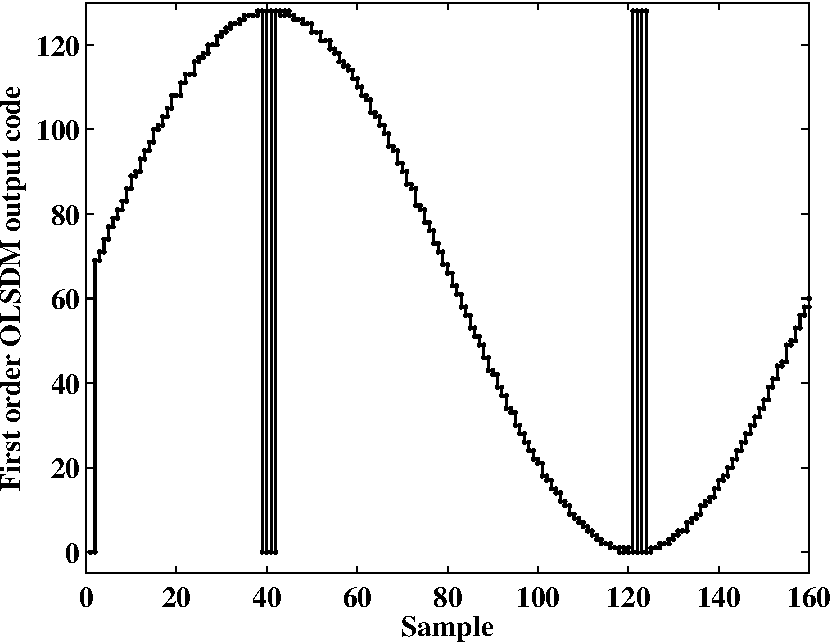
\includegraphics[width=\myfigwidth]{graphics/matolsdmerror} }
\caption{The output of the first order OLSDM in the presence of {\em false modulo} errors}
 \label{p4fig:matolsdmerror}
\end{figure}

%------------------------------------------------------
\subsection{Quantizer Linearity And Correction Of False Modulo Errors}\label{p4falsemodulo}
%------------------------------------------------------
An important issue of the amplitude modulated OLSDM is how the
linearity of the quantizer affects the system. 
The step sizes in the quantizer were made dependent on the
input signal, thus introducing a non-linearity.  By changing the
dependence on the input signal we control the linearity of the
quantizer. In this example an 7 bit quantizer with a maximum of 6.8
bit linearity was used as the quantizer in the second order OLSDM.
The results are presented for two different input amplitudes, $0.8FSR$
and $0.9FSR$. Figure \ref{p4fig:matlinolsdm2} shows
the linearity of the OLSDM as a function of quantizer
linearity. 
As expected, the linearity of the OLSDM does depend on the linearity
of the quantizer. For each bit of reduction in the linearity of the
quantizer the second order OLSDM looses half a bit of linearity. The
slope is constant until a threshold is reached, the threshold marks
the onset of {\em false modulo} errors. Below this threshold the SNDR
of the OLSDM degrades rapidly. The threshold is highly dependent on
the input amplitude and is on the order of \req{inputlimit2}.  Such a sharp
decrease in SNDR at a particular input signal amplitude is undesirable,
and it would be advantageous to correct for the cause of the sharp
degradation,  the {\em false
  modulo} errors.  As mentioned we can use the comparator output from
the analog modulo integrators to control modulo differentiation, which
will remove the {\em false modulo} errors. However, there is an alternate solution.

\begin{figure}[htbp]
\centerline{ 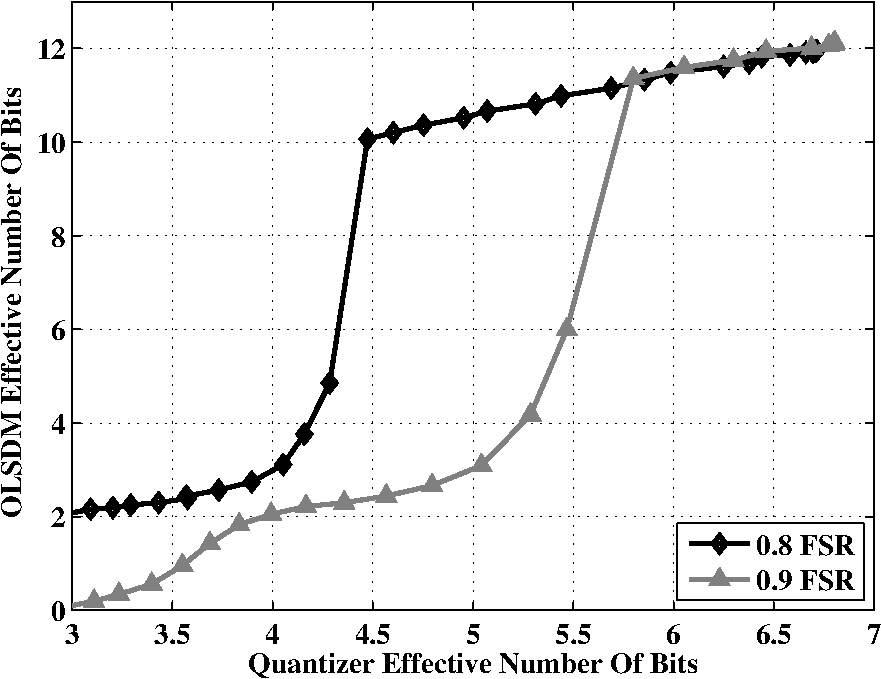
\includegraphics[width=\myfigwidth]{graphics/matlinolsdm2} }
\caption{Linearity of second order OLSDM as a function of quantizer linearity}
 \label{p4fig:matlinolsdm2}
\end{figure}

The {\em false modulo} errors have a large amplitude and high
frequency, as seen in Figure \ref{p4fig:matolsdmerror}. They span the
range of the output codes in two samples, and thus have a frequency
close to the Nyquist frequency. If we take advantage of the fact that
the input signal is, by choice, at least eight times lower than the
Nyquist frequency, since we chose an OSR of eight,  we can reduce the
errors. There is a maximum difference between two adjacent output
codes, which depend on the input signal. We assume a sinusoidal input
at one-eight of the Nyquist frequency. A sinusoid has a maximum slope
at the zero crossing which is approximately given by 
\eqn{
\label{p4eq:slopein}
 Slope  \approx A\pi/OSR
}, where A is the amplitude. In (\ref{p4eq:slopein}) we have used 
the well known assumption that $ \sin{x} \approx x $ if $x$ is
small and that $OSR = f_s/2f_{in}$. With an OSR of eight $Slope
\approx 0.39$ at zero crossing, which  is approximately one fifth of the FSR. 


We assume that any change in the output of more than $0.6FSR$ between
two consecutive samples is due to a {\em false modulo} error. 
If two consecutive samples of the OLSDM output has a difference of
more than 0.6FSR we undo the modulo operation. The result of this
simple correction can be seen in Figure
\ref{p4fig:matlinolsdm2corr}. The
error correction compensates for the dependence on input signal
amplitude and the onset of {\em false modulo} errors. It should be
noted that this error correction technique now allows the input
signal amplitude to be FSR.  

In this error correction technique we have made an assumption on the
properties of the output signal of the modulator. In this
assumption we must be cautious of the quantization noise. If we use a low
resolution quantizer the quantization noise power at higher frequencies can
be significant, and output codes which span the range of output codes
in two samples are certainly possible. Having said that, with higher
resolution quantizer and low order noise shaping the quantizer noise
power is not significant enough to influence the error correction.

\begin{figure}[htbp]
\centerline{ 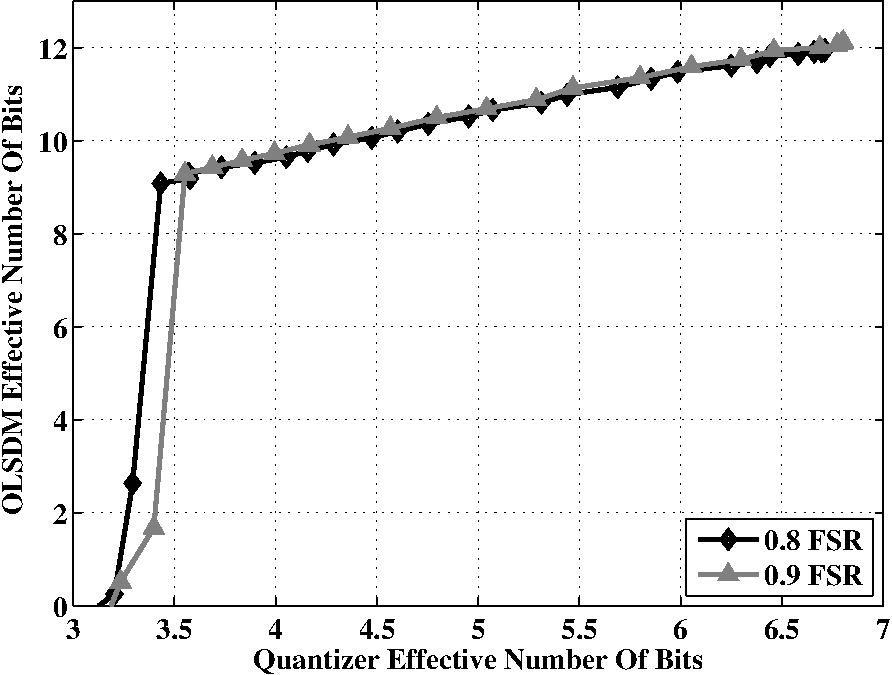
\includegraphics[width=\myfigwidth]{graphics/matlinolsdm2corr} }
\caption{Linearity of second order OLSDM as a function of quantizer
  linearity with error correction enabled} 
 \label{p4fig:matlinolsdm2corr}
\end{figure}

The circuit implementation of an amplitude modulated OLSDM requires an
analog modulo integrator. The next section explains how such a
function can be implemented by a switched-capacitor circuit.


%-------------------------------------------------------
\section{The Analog Modulo Integrator} \label{p4modint}
%-------------------------------------------------------
A requirement set on the
analog modulo integrator was that it should use maximum
swing available, for example 0.8V peak-to-peak with 1.2V supply. It should also be
a discrete time system and it should be amplitude modulated and not 
frequency modulated as was used in \cite{hovin97} and
\cite{wismar06}. The discrete time equation for a 
analog modulo integrator was shown in \req{modint}.

Using pseudo code the modulo integrator can be described as
\begin{enumerate}
\item Add the previous output to the current input
\item If the new output is equal to or exceeds the reference voltages
\item Subtract/Add the range of the integrator, $V_r$ 
\item Set the current output to the remainder
\end{enumerate}

A modulo operation is trivial to implement in the digital domain, but it may not be obvious how it
should be implemented in the
analog domain. Adding two voltages in the analog domain is conceptually
trivial. Whether a voltage exceeds a reference can be detected using a
comparator. Subtraction in the analog domain is also trivial, but
keeping the remainder presents a challenge. 

Assume that the reference voltages are
symmetric around the common mode, such that $|V_{ref}| =
|-V_{ref}|$ and $|V_{ref}|+ |-V_{ref}| = V_r$. The maximum internal
voltage in the modulo integrator  
would be less than $V_{ref} + V_{ref} = V_r$ or more than $-V_{ref} +
-V_{ref} = -V_r$.  So the output after 
summation, but before modulo operation, will be bounded by
\eqn{
\label{p4eq:brange}
-V_r < b(n) < V_r
}
In a circuit where the analog value is represented by voltages the
swing would have to be $2V_r$ to 
accurately represent all analog values. Since our input signal has a range
of $V_r$ we would waste an extra range of $V_r$ just to represent
intermittent values in the integrator. It would be better if we could
set the voltage swing of the circuit to $V_r$, which is equal to the
maximum input swing. But in a circuit where the analog values are
represented with voltages this is difficult.

%-------------------------------------------------------
\subsection{A Solution Based On Switched Capacitors}
%-------------------------------------------------------
Switched-Capacitor (SC) circuits are prevalent in many analog
integrated circuits. In discrete time \SD modulators it is common to
implement the integrator with a switched-capacitor circuit. It turns out that with small
modifications a switched-capacitor integrator can be converted to an analog modulo integrator. 

In switched-capacitor circuits the analog values are represented by
voltages across charged capacitors. A conventional
switched-capacitor integrator, shown in Figure \ref{p4fig:integrator}, adds the previous
output and current input. 

This simple integrator has two phases, sample ($\phi 1$) and charge
transfer ($\phi 2$). Assume the charge stored on $C_2$ is zero ($Q_2 = 0$). In the
sample phase we charge $C_1$ to the input voltage, thereby placing a
charge of $Q_1 = V_{i}C_1$ on the capacitor. During charge transfer
the charge of $C_1$ is transferred to $C_2$ by forcing the voltage
$V_g$ to be equal to ground using an operational amplifier. The
voltage across $C_1$ is then zero and there is no charge stored across
it, all charge is across $C_2$. This causes the output voltage to be
$V_o(n) = Q_1/C_2$. If the input value is kept constant, the next output
value, after a clock cycle, will be $V_o(n+1) = 2Q_1/C_2$. 

In the charge transfer phase $V_g$ is a high
impedance node, thus the total charge, $Q_{tot}$, given by $Q_{tot} = Q_1
+ Q_2$, does not change. $Q_{tot}$ is independent of the voltages at $V_g$ and
$V_o$. Thus we can argue that the ideal output value, $V_{o-ideal} =
Q_{tot}/C_2$ is only dependent on the total charge across the capacitors. By
ideal output voltage $V_{o-ideal}$ we mean the output voltage $V_o$ if
$V_g$ was forced to ground.

A real world operational amplifier
will normally have a maximum output signal swing. For example, if we exceed this signal swing the
gain in the operational amplifier goes down, and it is unable to force
virtual ground. In this case $V_o$ saturates, it cannot go any
higher, hence $V_o < V_{o-ideal}$. This saturation voltage we
define as $V_{sat} > V_{ref}$. 

Assume that the operational amplifier saturates in $\phi 2$, hence
$V_o = V_{sat} > V_{ref}$. If we can detect this condition, $V_o >
V_{ref}$, we can subtract a charge from $V_g$ that represents $V_r$
($V_r = 2V_{ref}$ as defined in Section \ref{p4modolsd}), thus
perform a modulo operation. We would now have \[V_{o-ideal} = (Q_{tot}-
Q_{V_r})/C_2 <
V_{ref} < V_{sat}\] as a consequence the operational amplifier will be
able to force virtual ground. 

One of the differences between the switched capacitor analog modulo
integrator and the conventional integrator is that the latter has three clock
phases. The first two have the same function as in the conventional
integrator, sample and charge transfer. The third clock phase is added
to detect if $V_o > V_{ref}$ (and the opposite, $V_o < -V_{ref}$) in phase two.
 If it does exceed, a charged capacitor
is connected to 
the charge transfer node of the integrator, node $V_g$ in Figure
\ref{p4fig:integrator}. This subtracts or adds the charge 
which represent $V_r$. This will change the charge transfer equation,
and as we shall see, implement a modulo operation. 

Provided that the input signal limited as specified by \req{inputlimit2}, the
subtracted/added charge will ensure that 
\eqn{
- V_{ref} < V_o < V_{ref}
}

\begin{figure}
\centerline{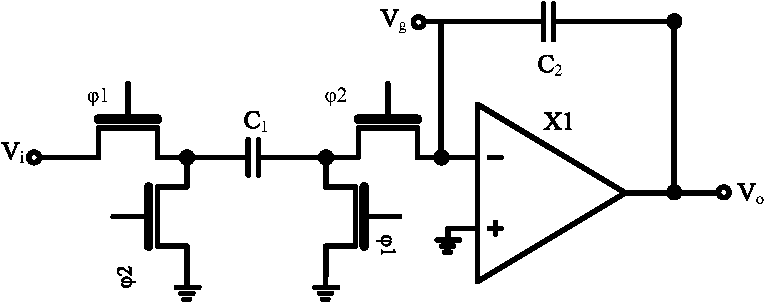
\includegraphics[width=\myfigwidth]{graphics/integrator}}
  \caption{Conventional switched capacitor integrator}
  \label{p4fig:integrator}
\end{figure}

The circuit needed to implement a modulo integrator is shown in Figure
\ref{p4fig:moddetector}. It is connected to the integrator in node $V_g$ and
$V_o$.
The complete circuit has, as mentioned,
three clock phases; $\phi 1$, $\phi 2$ and $\phi 3$. The timing
diagram is shown in Figure \ref{p4fig:timing}, where $T$ denotes the
period and $1/3, 2/3$ denotes the fractional time steps.  

\begin{figure}
\centerline{ 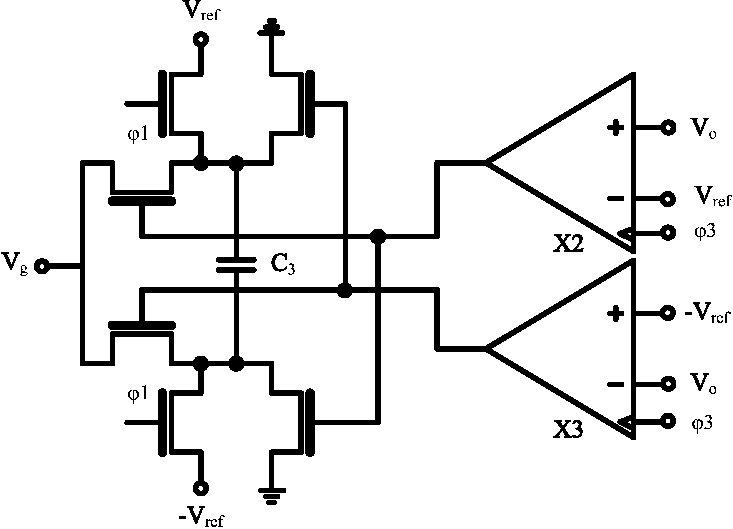
\includegraphics[width=\myfigwidth]{graphics/moddetector}}
  \caption{Modulo circuit}
  \label{p4fig:moddetector}
\end{figure}

\begin{figure}
\centerline{ 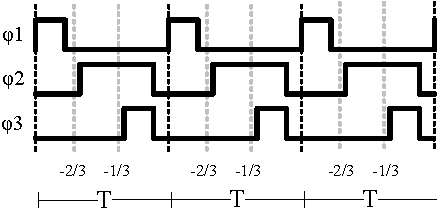
\includegraphics[width=\myfigwidth]{graphics/timing}}
  \caption{Timing diagram for the modulo integrator}
  \label{p4fig:timing}
\end{figure}


Consider the integrator in Figure \ref{p4fig:integrator}. During clock phase $\phi 1$ the
input signal is sampled across capacitor C1. In clock phase $\phi
2$, before $\phi 3$, the charge from C1 is transferred to C2. The charge transfer
equation will be 
\eqn{
\label{p4eq:chargetf1}
C_2V_o(n-T/3) = C_2V_o(n-T) + C_1V_i(n-2T/3)
}
In this equation, $V_o(n-T/3)$, is equivalent to
$ b(n)$ from equation \req{modintb} and will have the same bounds, assuming $C_1 = C_2$. For the 
output, $V_o(n)$,  to stay within the reference voltages, $V_r$ has to be
added or subtracted as in equation \req{modint}.

\begin{figure*}
\centerline{ 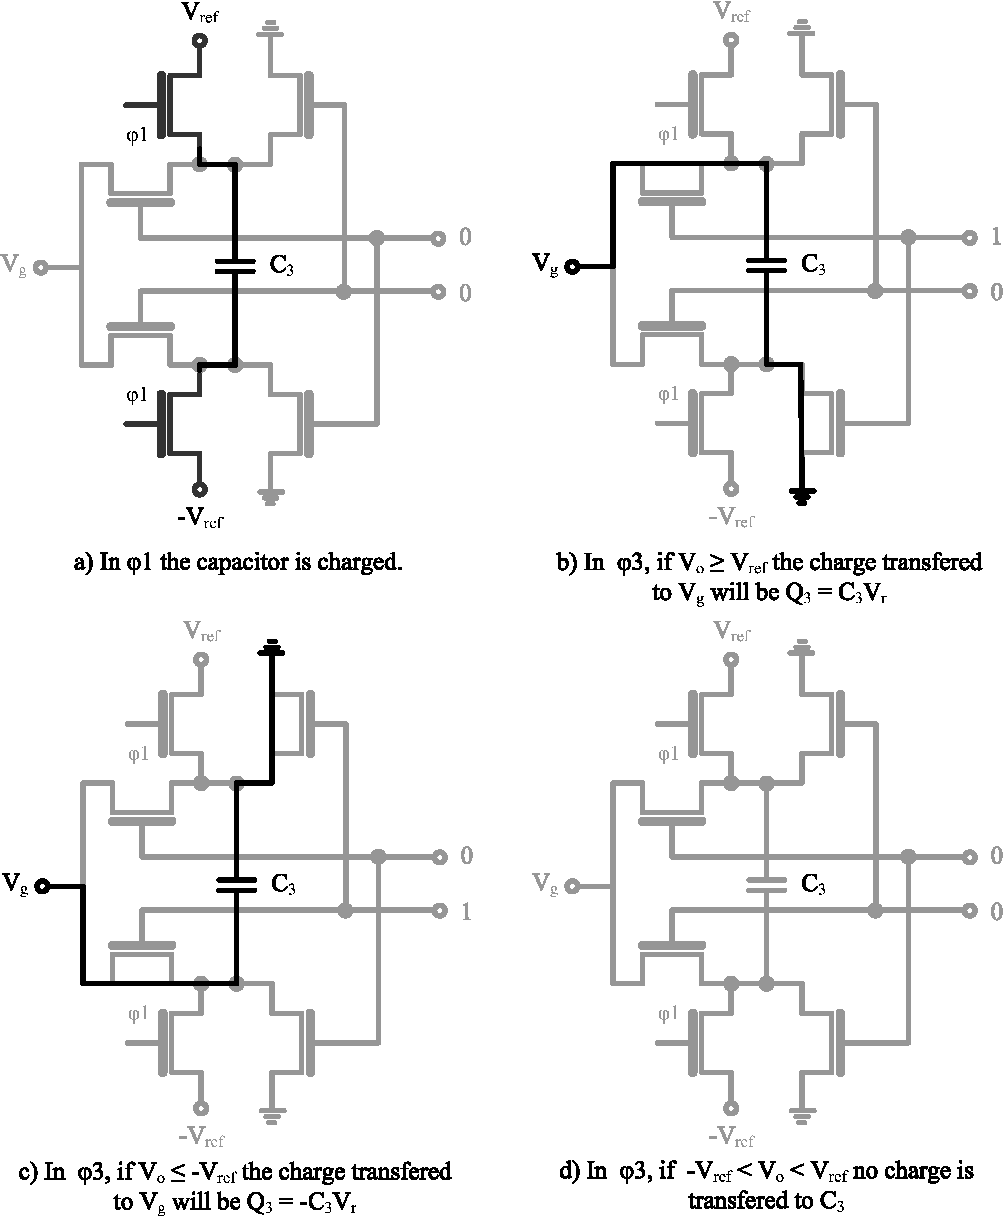
\includegraphics[width=5.5in]{graphics/moddetexpl}}
  \caption{The states of the modulo circuit in Figure \ref{p4fig:moddetector}}
  \label{p4fig:states}
\end{figure*}

Figure \ref{p4fig:states} shows the states of Figure \ref{p4fig:moddetector} in more detail. During $\phi 1$, Figure
\ref{p4fig:states} a) , the capacitor $C_3$ is charged to $V_r =
V_{ref} - -V_{ref}$. At the start of $\phi 3$ the latched comparators ( $X2$
and $X3$ in Figure \ref{p4fig:moddetector})
determine whether the output voltage exceeds the reference. Figure
\ref{p4fig:states} b) shows the connections if the
output voltage, $V_o(n-T/3)$, is higher than $V_{ref}$. Here a charge
of $Q_3 = C_3V_r$ is transferred to the node $V_g$ in the
integrator. This will change the charge transfer equation into
\eqn{
\label{p4eq:chargetf2}
C_2V_o(n) = C_2V_o(n-T) + C_1V_i(n-2T/3) - C_3V_r
}
For $V_o(n-T/3)$ lower than $-V_{ref}$, Figure \ref{p4fig:states} c) , the polarity of the charge is reversed and the charge transfer
function is
\eqn{
\label{p4eq:chargetf3}
C_2V_o(n) = C_2V_o(n-T) + C_1V_i(n-2T/3) + C_3V_r
}
And if $-V_{ref} < V_o(n-T/3) < V_{ref}$ the capacitor $C_3$ is not
connected to $V_g$ and the charge transfer function \req{chargetf1}
remains unchanged as shown in Figure \ref{p4fig:states} d). Notice that the outputs from the comparators can
never be high at the same time.

Combining the three equations,
\req{chargetf1}, \req{chargetf2} and \req{chargetf3} with $C_1 = C_2 = C_3$ and ignoring the
fractional time-steps ( $n-T/3$ and
$n-2T/3$) the result is \req{modint}.

The analog modulo integrator presented here resemble a first-order low
pass 1.5 bit 
\SD Modulator. If one plots the spectrum of the combined comparator
outputs it is a quantized first order noise shaped version of the
input. What
makes an analog modulo integrator different from a
first order low pass \SD Modulator is
\begin{itemize}
\item The quantizer levels are set at $\pm V_{ref}$, and not evenly
distributed between $\pm V_{ref}$. 
\item The three phase clock implements a
form of zero time quantizer 
feedback, if $V_o$ is higher than $V_{ref}$ $V_r$ is immediately
subtracted before the next output of the integrator.
\item The comparator outputs are not necessary to reverse the effect
  of the modulo operation in the digital domain.
\end{itemize}




%-------------------------------------------------------
\section{Behavioral Level Verification Of The SC OLSDM} \label{p4simulation}
%-------------------------------------------------------
We implemented a macro model description of the SC analog modulo
integrator described in the previous section.\footnote{The SPICE
  macro model of the switched capacitor analog modulo integrator can
  be downloaded from http://www.nextgenlab.net/olsdm} A single pole 
operational amplifier macro model
with a dc gain of 74dB and a voltage limiter was used to model
the operational amplifier. The comparators were modeled as latched
comparators. Ideal 
switches with an on resistance of 200 Ohms were used and the
capacitors C1-C3 were 5pF. The reference voltages
were $V_{ref} = 1V$ and $-V_{ref} = -1V$. The switch resistance, capacitance
and references were chosen arbitrarily. The output of the
operational amplifier was limited to $\pm 1.4V$. This ensures that for
some values of the input the integrator will saturate during $\phi
2$. The input frequency,
sampling frequency and the number of samples was the same as for the
Matlab simulation. An overview of the system can be seen in
Figure \ref{p4fig:matspice}. 

\begin{figure}[htbp]
\centerline{ 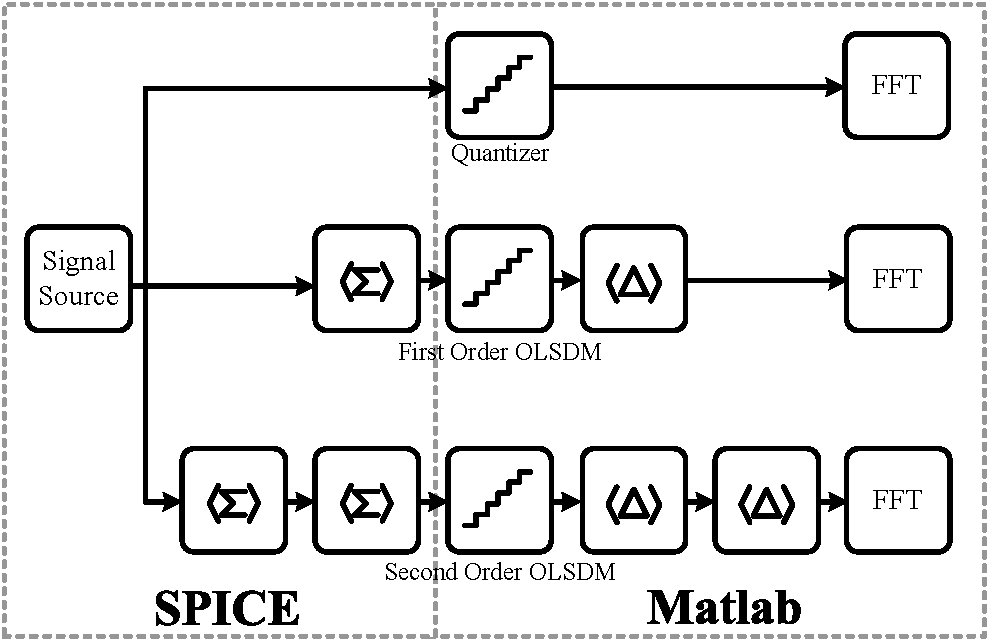
\includegraphics[width=\myfigwidth]{graphics/matspice}}
  \caption{Overview of circuit simulation with macro models}
  \label{p4fig:matspice}
\end{figure}

Only the analog modulo integrator was implemented in SPICE. Its output
was extracted and post-processed in Matlab. The code for the
differentiator and the quantizer were the same as in the behavioral
simulations. 

In Figure \ref{p4fig:modintsine} the input signal (dark gray) and the
output signal (light gray) of the first order SC modulo integrator is shown for
the first 150 samples. The sinusoidal input had an amplitude of $0.9
V$. The output, $V_o$, has 
been sampled at the end of $\phi 3$ and it can be seen how it never
exceeds the references at $V_{ref}$ and $-V_{ref}$.

\begin{figure}[htbp]
\centerline{ 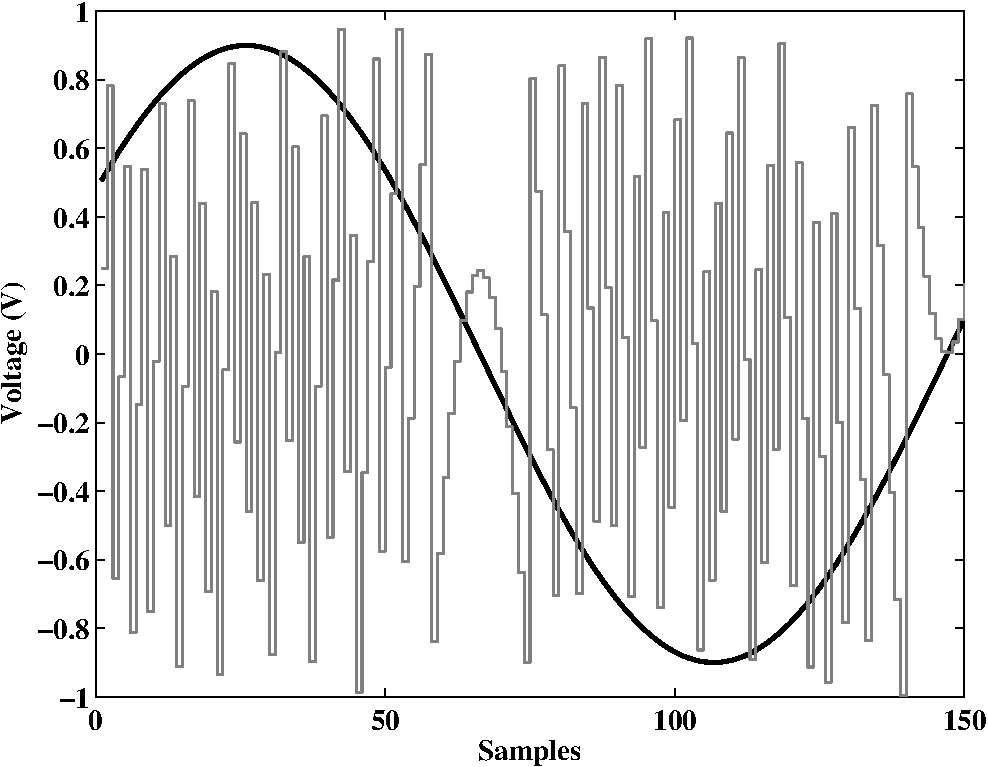
\includegraphics[width=\myfigwidth]{graphics/modintsine}}
  \caption{Input vs output for the modulo integrator. Input is a sine
  with an amplitude of 0.9 V}
  \label{p4fig:modintsine}
\end{figure}

A transient simulation was performed. The results are summarized
in Table \ref{p4tab:olsdmsndrspice}. If we remove the effect of reduced
input signal amplitude the errors are $-0.2dB$ for first order OLSDM
and $-2.1dB$ for second order OLSDM. The error for first order OLSDM
is within the error of the SNDR extraction. The error for the second
order OLSDM it is to large to be caused by deviations due to SNDR
extraction. This extra loss of $-2.1dB$ was mainly due to non-linearity
of the voltage limiter used in the simulation. When the voltage
limiter is removed the error for second order OLSDM is reduced to
$-0.79dB$. The remaining difference is mostly due to finite gain in the
operational amplifier. The FFTs of the first and second order OLSDM are
shown in Figure \ref{p4fig:olsdmspice} and Figure \ref{p4fig:olsdmspice2},
the ideal quantizer in light gray and the OLSDM output in dark gray. 

\begin{table}[htbp]
\caption{ SNDR of OLSDM modulators in SPICE}
\begin{tabular}{cccc}
\label{p4tab:olsdmsndrspice}
 Noise Shaping & Total (dB) & Difference from Ideal (dB)\\ 
\hline 
First order &  64.7 & -1.1 \\ 
Second order & 73.1 & -3 \\ 
\end{tabular} 
\end{table}

 \begin{figure}[htbp]
\centerline{ 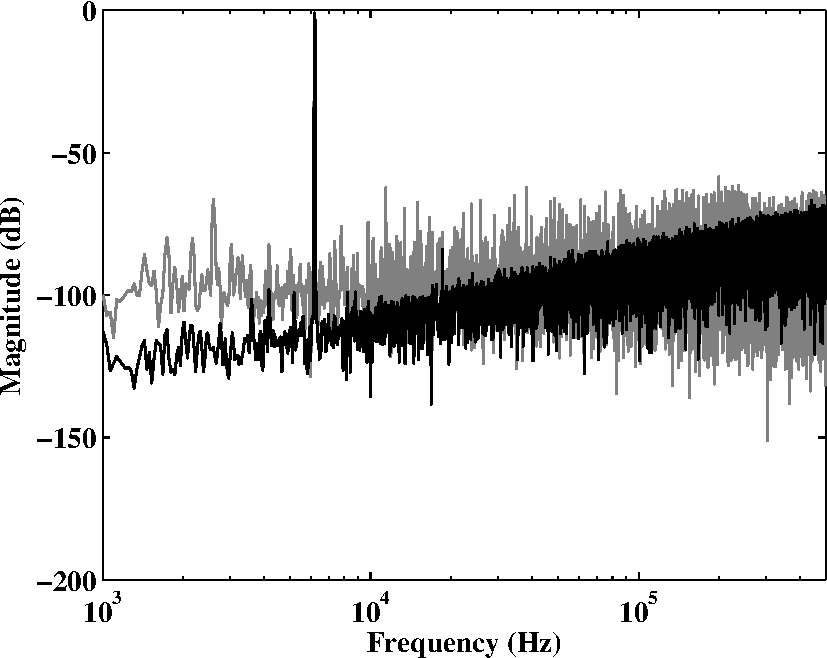
\includegraphics[width=\myfigwidth]{graphics/olsdmspice}}
 \caption{FFT of output from first order OLSDM simulation in SPICE.}
 \label{p4fig:olsdmspice}
\end{figure}

 \begin{figure}[htbp] 
\centerline{ 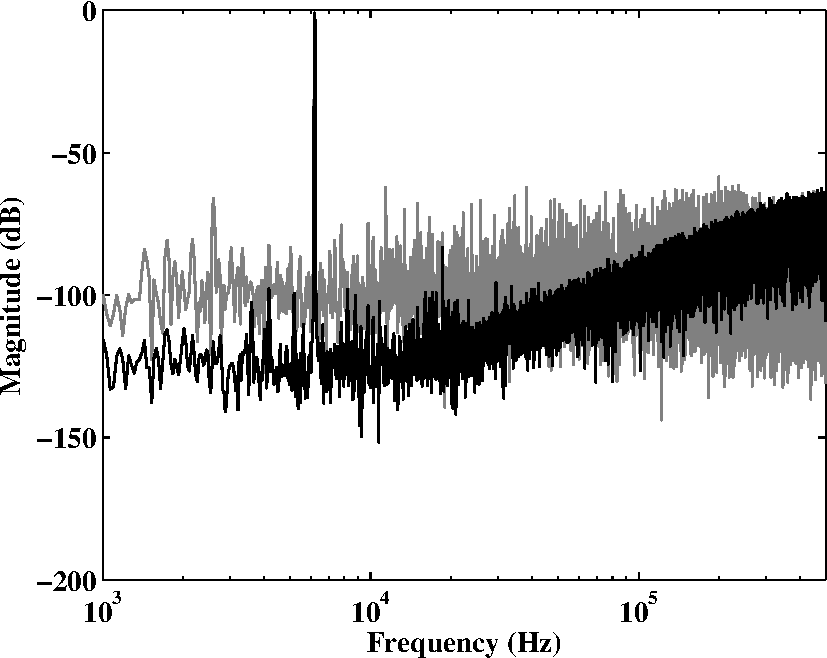
\includegraphics[width=\myfigwidth]{graphics/olsdmspice2}}
 \caption{FFT of output from second order OLSDM simulation in SPICE.}
 \label{p4fig:olsdmspice2}
\end{figure}


%-------------------------------------------------------
\section{Future Work}
%-------------------------------------------------------
There are no integrated circuit implementations of an amplitude
modulated OLSDM as of
yet. An integrated circuit implementation would be the next step. It
is needed to check whether the amplitude modulated OLSDM has a place in the
family of analog-to-digital converters, or whether it is just of
academic interest. There are many questions to be 
answered and some questions that have not yet been asked. The
switched capacitor analog modulo integrator is, to our knowledge, new 
circuit, and it may find applications outside the realm of OLSDM.  
 
%-------------------------------------------------------
\section{Conclusion}
%-------------------------------------------------------
We introduced the switched capacitor analog modulo integrator, which
to our knowledge is a new circuit. We introduced
the amplitude modulated open loop \SD modulator (OLSDM), which is an analog modulo integrator
followed by a quantizer and a modulo differentiator. The mathematical
equivalence between low pass \SD modulators and OLSDM was
explained. Behavioral simulations confirmed the equivalence. The
necessary circuit, a switched capacitor analog modulo integrator, was explained in detail. 
Behavioral level simulations in SPICE of the analog modulo
integrator verified the function, and proved the concept of
amplitude modulated OLSDM.

%------------------------------------------------------------------------
%\begin{acknowledgements}
%------------------------------------------------------------------------
\section*{Acknowledgments}
 Financial support from the Norwegian Research Council through the
project Smart Microsystems for Diagnostic Imaging in Medicine (project
number 159559/130) and the project ASICs for Microsystems (project
number 133952/420) is gratefully acknowledged.
%\end{acknowledgements}




%\bibliography{IEEEabrv,wulff}

% \begin{thebibliography}{00}

% \bibitem{Widrow56}
% Widrow, B.: 1956, `A Study of Rough Amplitude Quantization by Means of Nyquist
%   Sampling Theory'.
% \newblock {\em Circuit Theory, IRE Transactions on} {\bf 3}(4), 266--276.

% \bibitem{claasen80}
% Claasen, T. A. C.~M., W.~F.~G. Mecklenbraucker, J.~B.~H. Peek, and N. van
%   Hurck: 1980, `Signal Processing Method for Improving the Dynamic Range of A/D
%   and D/A Converters'.
% \newblock {\em {IEEE} Trans. Acoust., Speech, Signal Processing} {\bf 28}(5),
%   529--538.


% \bibitem{hovin97}
% H{\o}vin, M., A. Olsen, T.~S. Lande, and C. Toumazou: 1997, `Delta-Sigma
%   Modulators Using Frequency -Modulated Intermediate Values'.
% \newblock {\em {IEEE} J. Solid-State Circuits} {\bf 32}(1), 13--22.

% \bibitem{wismar06}
% Wismar, U., D. Wisland, and P. Anderiani: 2006, `A 0.2V 0.44 �W 20 kHz Analog
%   to Digital Modulator with 57 fJ/conversion FoM'.
% \newblock In: {\em Proc ESSIRC'06}, Vol.~1. pp. 187--190.


% \bibitem{wisland02}
% Wisland, D.~T., M.~E. H{\o}vin, L.~A. Fleischer, and T.~S. Lande: 2002a, `A new
%   scalable non-feedback sigma-delta Digital-to-Analog Converter'.
% \newblock In: {\em Proc. ICECS'02}, Vol.~1. pp. 331--334.

% \bibitem{brooks97}
% Brooks, T.~L., D.~H. Robertson, D.~F. Kelly, A.~D. Muro, and S.~W. Harston:
%   1997, `A Cascaded Sigma-Delta Pipeline A/D Converter with 1.25MHz Signal
%   Bandwidth and 89 dB SNR'.
% \newblock {\em {IEEE} J. Solid-State Circuits} {\bf 32}(12), 1896--1906.


% \bibitem{johns}
% Johns, D. and K. Martin: 1997, {\em Analog Integrated Circuit Design}.
% \newblock John Wiley \& Sons, Inc.



% \bibitem{IEEE-1241}
% IEEE: 2001, `IEEE standard for terminology and test methods for
%   analog-to-digital converters'.
% \newblock IEEE Std 1241-2000.


% \bibitem{wisland02a}
% Wisland, D.~T., M.~E. H{\o}vin, L.~A. Fleischer, and T.~S. Lande: 2002b, `A
%   second-order non-feedback /spl Delta//spl Sigma/ modulator for D/A
%   conversion'.
% \newblock In: {\em Proc. ICECS'02}, Vol.~1. pp. 327--330.


% \end{thebibliography}

%\input{authors.tex}

%\begin{vitae}



%\centerline{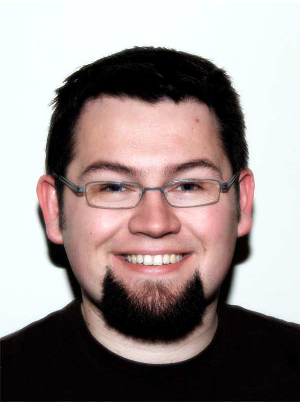
\includegraphics[width=20mm]{wulff-photo} }
%\Vauthor{Carsten Wulff}
%\begin{figure}[h]

%\end{figure}
% \textbf{Carsten Wulff}
%%received the M.Sc degree in electrical engineering from the Department
%of Physical Electronics, Norwegian University of Science and
%Technology (NTNU), in 2002. He was employed as a research assistant
%at NTNU during 2003-2004. Since 2004 he has been working towards his PhD. In
%2006-2007 he was a visiting researcher at Department of Electrical and
%Computer Engineering, University of Toronto. 
% His present research interest include analog and mixed-signal
%CMOS design, and design of analog-to-digital converters with a
%particular focus on comparator based switched capacitor circuits.   

%\Vauthor{{\O}ystein Knauserud}
%\textbf{{\O}ystein Knauserud}
%received the M.Sc degree in electrical engineering from the Department of Electronics and Telecommunication, Norwegian University of Science and Technology (NTNU), in 2006. He is currently at ARM, Embedded Graphics Solutions in Trondheim, Norway.


%\begin{figure}[h]
%\centerline{
\includegraphics[width=20mm]{trond} }
%\end{figure}

%\textbf{Trond Ytterdal}
%\Vauthor{Trond Ytterdal}
%received his M.Sc. and Ph.D. degrees in electrical
%engineering from the Norwegian Institute of Technology in 1990 and 1995,
%respectively. He was employed as a research associate at the Department of
%Electrical Engineering, University of Virginia (1995-1996) and as a research
%scientist at the Electrical, Computer and Systems Engineering Department,
%Rensselaer Polytechnic Institute in Troy, New York (1996-1997). From 1997 to
%2001 he worked as a senior ASIC designer at Nordic Semiconductor in
%Trondheim, Norway. In 2001 he became a Professor at the Department of
%Electronics and Telecommunication, Norwegian University of Science and
%Technology (NTNU). Prof. Ytterdal's present research interests include
%design of analog integrated circuits, behavioral modeling and simulation of
%mixed-signal systems, modeling of nanoscale transistors and novel device
%structures for application in circuit simulators. He has published more than
%100 scientific papers in international journals and conference proceedings.
%He is a co-author of the books Semiconductor Device Modeling for VLSI
%(Prentice Hall, 1993), Introduction to Device Modeling and Circuit
%Simulation (Wiley, 1998) and Device Modeling for Analog and RF CMOS Circuit
%Design (Wiley, 2003), and has been a contributor to several other books
%published internationally. He is also a co-developer of the circuit
%simulator AIM-Spice. Prof. Ytterdal is a member of The Norwegian Academy of
%Technological Sciences and a Senior Member of IEEE.




%\end{vitae}


%\end{document}
